\chapter{Mesh-sweeping for sparse manifold refinement}





\section{Introduction}
\label{sec:intro}
Reconstructing the observed scene from a set of images is a widely studied problems in computer vision: it is known as \emph{Structure from Motion} (SfM), when the aim is to reconstruct both the scene (the structure) and the camera poses (the motion), or as \emph{multi-view stereo} (MVS), when camera poses are known.
While SfM techniques provide a sparse reconstruction of the environment, MVS aims at reconstructing a dense and accurate model of the observed scene. 

Since the datasets of \cite{Seitz_et_al06} and \cite{strecha2008} were made available, dense MVS has been faced with different approaches, some of which reaching very accurate results, but some issues are still open, e.g., the initialization and the management of untextured regions and false matches.
According to the kind of representation of the 3D model, MVS techniques can be subdivided in \emph{point-based}, \emph{volumetric-based} and \emph{mesh-based} methods.
Point-based methods estimate the depth of each image pixel, reconstructing a point cloud \cite{fu10,Tola12}; they provide accurate and dense point clouds, but the outcome is often redundant where the surface is flat, and they are not able to reconstruct untextured area.
Volumetric-based methods, first proposed by \cite{curless1996volumetric}, build the reconstruction by discretizing the space and labeling as matter or free space the voxels as in \cite{curless1996volumetric} or the tetrahedra as in \cite{labatut2007efficient}.
Voxel-based methods  require a huge amount of memory, and even if attempts to make the representation more compact exist \cite{steinbrucker2014volumetric}, they are still not suitable for scalable reconstruction.
Tetrahedron-based methods are more compact, but the accuracy of the reconstruction still needs to be refined to reach state-of-the-art results.
This latter approach is often used as an initialization to mesh-based methods in \cite{vu_et_al_2012,hiep2009towards,salman2010surface}.

Mesh-based methods have been proven to be suitable to build continuous, high accurate reconstructions of both small objects and large-scale scenes \cite{hiep2009towards,vu_et_al_2012,salman2010surface}.
These methods refine an existing mesh by minimizing an image similarity measure such as the Zero Mean Cross Correlation (ZNCC) \cite{hiep2009towards,pons2007multi,zaharescu2007transformesh} or the Sum of Squared Differences (SSD) \cite{delaunoy_et_al_08,delaunoy2011gradient}. 
The initialization of this existing mesh is one of the major issues in the state-of-the-art mesh-based MVS methods. For single object reconstruction, as in the Middelbury dataset \cite{Seitz_et_al06}, the initial mesh is usually estimated by the visual hull \cite{laurentini1994visual}, but this is not applicable in more complex scene such as the ones in \cite{strecha2008} or in large-scale scenarios.

One of the most effective and scalable mesh-based algorithm for multi-view stereo was proposed by Vu \emph{et al}. \cite{vu_et_al_2012}; in their work, the authors initialize the mesh evolution algorithm by extracting a very dense and noisy point cloud, building a Delaunay triangulation out of it, and estimating the initial mesh via a \emph{s-t} cut algorithm based on the work of \cite{labatut2007efficient}. 
This last work inspired other extensions such as \cite{jancosek2011multi}.
The main problem with this approach is that the \emph{s-t} cut does not guarantee the output mesh to be a manifold while the \emph{surface evolution} algorithm needs this property; indeed Vu \emph{et al}.  need to manually check the outcome of the \emph{s-t} cut before the surface evolution.

Some mesh-based algorithms, e.g., \cite{pan2015automatic,li2015detail}, initialize the reconstruction with a point-based MVS such as CMVS \cite{fu10} together with Poisson Reconstruction \cite{kazhdan2006poisson}.
This process automatically provides an initialization usually close to be manifold but not guaranteed, but it has issues related to redundancy of the points and non-scalability.


In the literature, some methods  to estimate a manifold mesh exist, but most of them rely on silhouettes \cite{vogiatzis2005multi,furukawa2006carved,esteban2004silhouette}, thus they are limited to small objects, or they are not scalable due to the usage of voxel-based reconstruction \cite{hornung2006hierarchical}.
A suitable approach to estimate a manifold mesh has been recently proposed in \cite{lhuillier_Yu2013,litvinov_lhuillier_13,Romanoni15a,Romanoni15b}: the authors incrementally reconstruct the scene from very sparse data which are the outcome of SfM algorithms. 
For many applications the reconstruction relying only on these points is sufficient, but for a surface evolution approach, needs resolution and accuracy improvements. Indeed, to avoid getting stuck in local minima during the evolution process, also Vu \emph{et al}. need to densify the point cloud extracted by the SfM algorithm.

In this paper we propose a novel and fully automatic approach to estimate a manifold, suitable for being a good initialization for a surface evolution mesh-based MVS algorithm.
We bootstrap from a manifold reconstructed in a similar fashion to \cite{litvinov_lhuillier_13}, and we refine it by iteratively sweeping the triangles of the manifold around their neighborhood looking for very good stereo matches.
This approach takes inspiration from the multi-directions plane-sweep of \cite{gallup2007real}.
In \cite{gallup2007real}, the authors sweep a set of planes choosing fixed directions related to the direction of the walls identified from Structure from Motion points; for each pixel and each plane they collect the matching costs among the views and choose the best stereo matching cost to estimate depth maps.
Another interesting method that performs local plane sweeping is presented in \cite{sinha2014efficient}, where, again, the output is a depth map.
In the proposed approach, instead, we estimate directly a manifold mesh; the directions of the planes are automatically driven by the data; and we avoid to sweep on the whole scene, since we look for new 3D points in the neighborhood of the iteratively reconstructed manifold. 
Differently from \cite{gallup2007real}, we directly recover a consistent dense 3D mesh instead of independent depth maps.

% \begin{figure}[t]
%   \centering
%   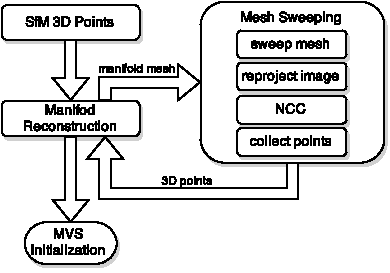
\includegraphics[width=0.9\columnwidth]{././img/meshSweeping.pdf}
% \caption{Overview of the proposed algorithm.}
%   \label{fig:overview}
% \end{figure}


In Section \ref{sec:manifold_ch6} we summarize the manifold reconstruction algorithm. 
In Section \ref{sec:sweep} we explain how we refine the initial manifold mesh obtained from the previous step. In Section sec:experimental we show the results of our approach, underlying the improvement of the reconstruction accuracy thanks to the sweeping algorithm on both simulated and real datasets In Section \ref{sec:conclusion} we conclude pointing out possible future work.
% 
% 
% \section{Related work}
% \label{sec:relwork}
% % Since the datasets of \cite{Seitz_et_al06} and \cite{strecha2008} were made available, dense MVS has been faced with different approaches, some of which reach very accurate results on these datasets, but some issues are still open, lack of texture and false matches above all.
% % According to the kind of representation of the 3D model, MVS techniques can be subdivided in \emph{point-based}, \emph{volumetric-based} and \emph{mesh-based} methods. 
% % 
% % Point-based methods often estimate the depth of each image pixel, reconstructing a point cloud. The most successful approaches find very accurate matches among the views and estimate their corresponding 3D position, then they expand the depth information to the corresponding neighborhood as in \cite{fu10} and \cite{Tola12}.
% % These methods provide very accurate and dense point clouds, but this kind of representation is often redundant where, for instance, the reconstructed surface is flat, and, at the same time, they are not able to reconstruct untextured or ambiguous area, when correspondences become difficult to estimate.
% % Moreover, for better visualization or in concerned applications in order to obtain a dense and continuous representation of the scene, they often need a meshing step, for instance Poisson Reconstruction, which can lead to artifacts or over-smoothed surfaces, due to some noise or missing data in the point cloud, and this step results non-scalable for large-scale scenes.
% % 
% % Volumetric-based methods, first proposed by \cite{curless1996volumetric}, build the reconstruction by discretizing the space and labeling as matter or free space the voxels as in \cite{curless1996volumetric} or the tetrahedra as in \cite{labatut2007efficient}.
% % The voxel-based methods  require a huge amount of memory, and even if attempts to make the representation more compact exist \cite{steinbrucker2014volumetric}, they are still not suitable for scalable reconstruction.
% % Moreover, only by including shape priors these methods are able to handle lack of texture \cite{karimi2015segment}.
% % The tetrahedron-based methods rely on a Delaunay triangulation built upon a point cloud, which is much more compact, but the accuracy of the reconstruction still needs a refinement to reach state-of-the-art results, indeed it is used as an initialization to mesh-based methods in \cite{vu_et_al_2012,hiep2009towards,salman2010surface}.
% % Those approaches end up in obtaining more robust results, compared to voxel-based approaches, in the presence of untextured regions: the Delaunay triangulation intrinsically adapts the dimensions of the triangulation to the point cloud, such that the facets of large tetrahedra cover the untextured regions, even if no matches among views are available.
% % 
% % Mesh-based methods have been proven to be suitable to build continuous, high accurate reconstructions of both small objects and large-scale scenes \cite{hiep2009towards,vu_et_al_2012,salman2010surface,vu2011large}.
% % These methods refine an existing mesh, estimated for instance,  upon the reconstruction performed by one of the previous methods; the refinement involves the minimization of an image similarity measure such as the Zero Mean Cross Correlation (ZNCC) \cite{hiep2009towards,pons2007multi,zaharescu2007transformesh} or the Sum of Squared Differences (SSD) \cite{delaunoy_et_al_08,gargallo2007minimizing,delaunoy2011gradient}. 
% % Even if the initialization relies on one of the previous approaches, mesh-based methods can estimate sub-maps and then merge them together as in \cite{vu2011large}, so that the large-scale reconstruction is feasible both on computational and memory sides.


\begin{figure}[t]
\centering
\begin{tabular}{ccc}
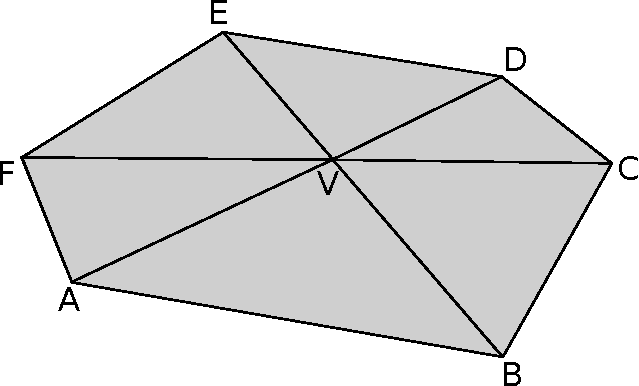
\includegraphics[width=0.28\columnwidth]{./img/manifold}&
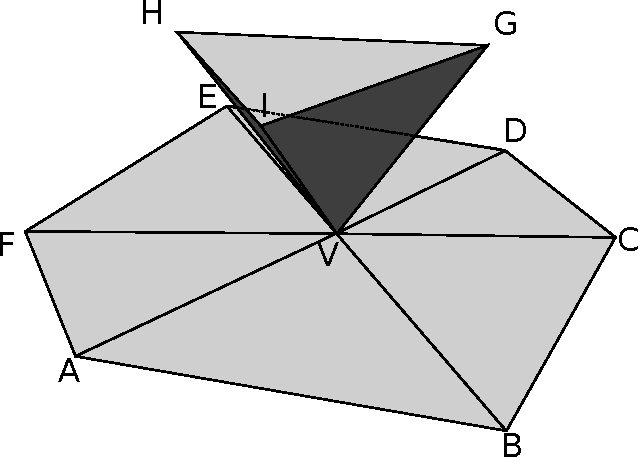
\includegraphics[width=0.28\columnwidth]{./img/notmanifold1}&
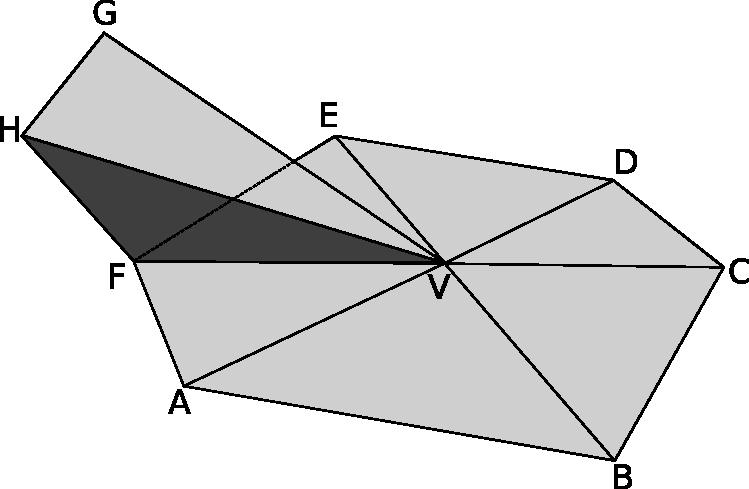
\includegraphics[width=0.28\columnwidth]{./img/notmanifold2}\\
(a)&(b)&(c)
\end{tabular}
\caption{The manifold property: the vertex $V$ in (a) is regular ($ABCDEF$ is a closed path without cycles), while in (b) and (c) the vertex $V$ is not regular since, in the former case the path $ABCDEFGHI$ is not closed, and in the latter $ABCDEFGHF$ has two cycles.}
\label{fig:vertexManifold}
\end{figure}


%------------------------------------------------------------------------- 
\section{Manifold Reconstruction}
\label{sec:manifold_ch6}
In the proposed system, we iteratively alternate manifold reconstruction and mesh sweeping.
Let recall that the manifold property holds if and only if the neighborhood of each surface point is homeomorphic to a disk. 
So a mesh, which is a discrete surface, is manifold if and only if each vertex $v$ is \emph{regular}, i.e., if and only if the edges opposite to $v$ form a closed path without loops  \cite{litvinov_lhuillier_13}. 
We show in Figure \ref{fig:vertexManifold} (a) one example of a regular vertex and in Figure \ref{fig:vertexManifold}(b) and \ref{fig:vertexManifold}(c) two cases where the vertices are not regular and thus break the manifold property.

In literature \cite{Hoppe13,litvinov_lhuillier_13}, reconstruction from sparse data involves the estimation of a mesh which usually partitions the 3D Delaunay Triangulation of the sparse points between two sets: free space and matter.
In this case the sources of non-manifoldness can be induced by tetrahedra intersecting at a vertex, and by tetrahedra with a common edge (non-manifold edge). 
In both cases the non-manifoldness can be fixed, in principle, by cloning and offsetting the vertex of intersection, but two big drawbacks arise: this process would invalidate the Delaunay property, that we need to keep valid in an incremental setting, and, since many non-manifold vertices are generated, rearranging the triangulation and the visibility information for each non-manifold point becomes inefficient. For these two reasons we need a different approach to enforce the manifoldness.

We reconstruct the first manifold with the algorithm proposed in \cite{litvinov_lhuillier_13}, slightly modified by a weighting scheme as in \cite{Romanoni15b}, bootstrapping from the camera poses, the points and the visibility estimated by a Structure from Motion algorithm\footnote{In our implementation we use VisualSFM \cite{wu2011visualsfm}.} .% that avoids the creation of most visual artifact in the final mesh (more discussion about visual artifacts in \cite{litvinov_Lhiuller14}). %TODO !!!!!!!!!!!!!!!!!!!! add cite Romanoni15a
The manifold is reconstructed such that it partitions the 3D triangulation of the SfM points, between the set $O$ of \emph{outside} tetrahedra, i.e., the subset of the free space outside the manifold (not all the free space tetrahedra will be part of the space outside the manifold), and the complementary set $I$ of inside tetrahedra (i.e. the remaining tetrahedra that represent the matter together with the free space tetrahedra which would invalidate the manifold property). A weight is associated to each tetrahedron and it keeps track of the visibility information, i.e., the camera-to-point viewing rays; in the following, a tetrahedron belongs to free space if its weight is higher than $t_w$ (in our case $t_w = 4.0$).



The manifold is obtained by four steps. (1)  \emph{Point Insertion}: build the 3D Delaunay triangulation of the 3D SfM points. (2) \emph{Ray tracing and tetrahedra weighting}: for each camera-to-point viewing ray, add a weight $w_1 = 4.0$ to the intersected tetrahedra and a weight $w_2=0.5$ to their neighboring tetrahedra.
Such weighting scheme acts as a smoother of the visibility and avoids the creation of visual artifacts (see \cite{litvinov_Lhiuller14} for a detailed discussion about visual artifacts). (3) \emph{Growing}: initialize a queue $Q$ starting from the tetrahedron with the higher weight. 
Then: (a) pick  the tetrahedron with highest weight from $Q$ and add it to $O$ only if the resulting surface between $O$ and $I$ remains manifold; (b) add the neighboring tetrahedra to the queue $Q$, otherwise discard it; continue iteratively until $Q$ is empty.
  

\subsection{Incremental refinement of the manifold}
In order to refine this initial mesh, we iterate between the mesh sweeping algorithm described in Section \ref{sec:sweep} that outputs a set $P$ of 3D new points, and the incremental reconstruction (this section)  until convergence is reached (i.e., no more points to be added or the number of iteration is greater than $it_{max} = 15$).

The insertion of a point $p\in P$  into the Delaunay triangulation causes the removal of the set $D$ of tetrahedra, breaking the Delaunay property. The surface between $O \setminus D$ and $I \cup D$ is not guaranteed to be manifold anymore. 
In order to avoid this, as the authors in \cite{litvinov_lhuillier_13}, we define a list of tetrahedra $E \supset D$ and apply the \emph{Shrinking} procedure, i.e., the inverse of Growing:  we subtract iteratively from $O$ the tetrahedra  $\Delta \in E$ keeping the manifoldness valid.
After this process, it is likely that $D \cap O = \emptyset$.
Whenever $D \cap O \neq \emptyset$ the point $p$ is not added to the triangulation and it is discarded.
Once all points in $P$ have been processed, the queue $Q$ is initialized with the tetrahedra $\Delta \in T \setminus O$ such that  $\Delta \cap \delta O \neq \emptyset$, and the Growing process starts as explained above.


\begin{figure}[tp]
  \centering
  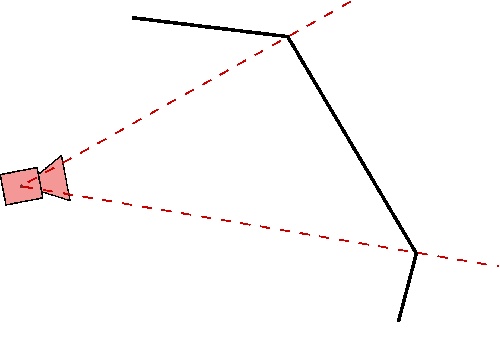
\includegraphics[height=0.3\textwidth]{././img/sweep.pdf}
  % sweep.pdf: 257x195 pixel, 72dpi, 9.07x6.88 cm, bb=0 0 257 195
  \caption{Example of manifold sweeping with respect to the camera $C$}
  \label{fig:sweep}
\end{figure}


 

%------------------------------------------------------------------------- 
\section{Mesh Sweeping}
\label{sec:sweep}
After each manifold reconstruction step, we apply the novel mesh sweeping algorithm to look for new 3D points in the neighborhood of the manifold mesh, which we assume to be close to the true model of the scene.
These points will be added to the reconstruction in the next manifold reconstruction step.

For each camera, we sweep the visible part of mesh $\mathcal{M}$ along the viewpoint direction (see Figure \ref{fig:sweep}). 
Given a camera located in $C$, we sweep each visible facet $f$ of $\mathcal{M}$ by an amount multiple of $\alpha$ (in our case $\alpha = 3$cm).
Let $v^1$, $v^2$ and $v^3$ be the vertices of $f$, and let $\theta^i$ be the angle between the normal $n$ of the facet and the ray $d^i$ from the camera center to the vertex $v^i$. 
The new vertex $v_j^i$ of the swept facet is now computed as:
$
v_j^i = v^i + \alpha_j \cdot \cos (\theta^i) \cdot d^i,
$
where $\alpha_j = \alpha \cdot k_j$, with $k_j \in \mathbb{N}$ and $-10< k_j <10$ is the distance swept (let note that is fixed for all the facets).

Since all the visible vertices of each triangle are swept by the same amount along the camera-to-point direction, no self-intersections among facets has been induced. 


% 
% \begin{figure}[t]
% \centering
% 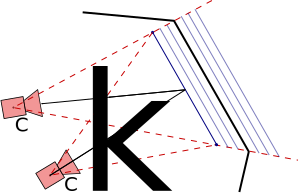
\includegraphics[width=0.3\textwidth]{./img/sweepSteps-01}
% \caption{Reprojection of image $I_k$ on camera $C$ through one of the mesh triangle.}
% \label{fig:stereo}
% \end{figure}

\begin{figure}[t]
  \centering
  \includegraphics[height=0.3\textwidth]{././img/matching.pdf}
\caption{3D points extraction process after the mesh sweeping.}
  \label{fig:matching}
\end{figure}

\begin{figure*}[th]
\setlength{\tabcolsep}{1px}
\centering
\begin{tabular}{ccccc}
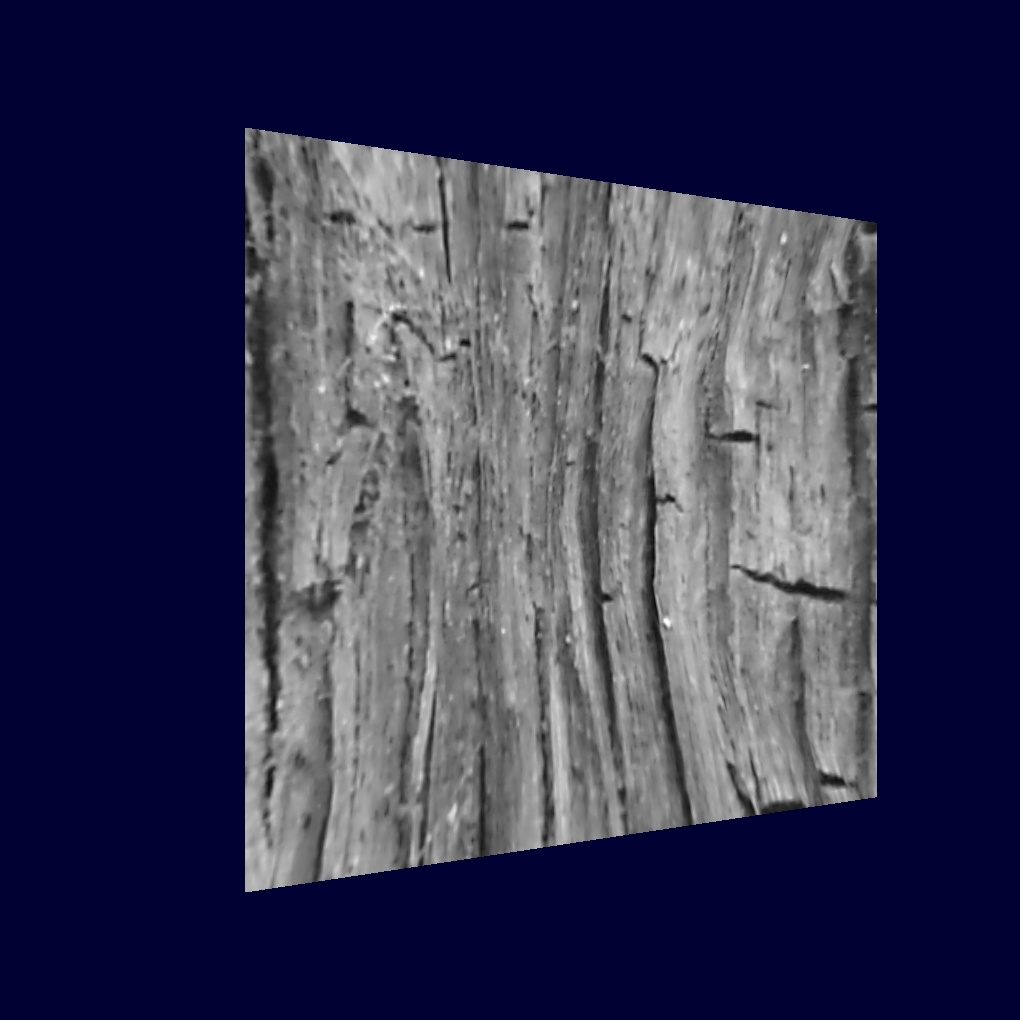
\includegraphics[height=0.18\textwidth]{./img/datasetSweepIMG0}&
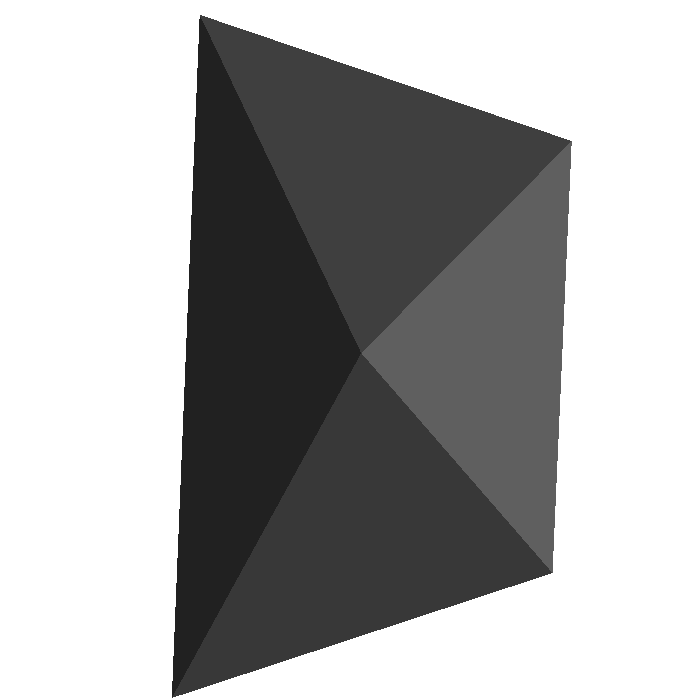
\includegraphics[height=0.18\textwidth]{./img/synthGT1}&
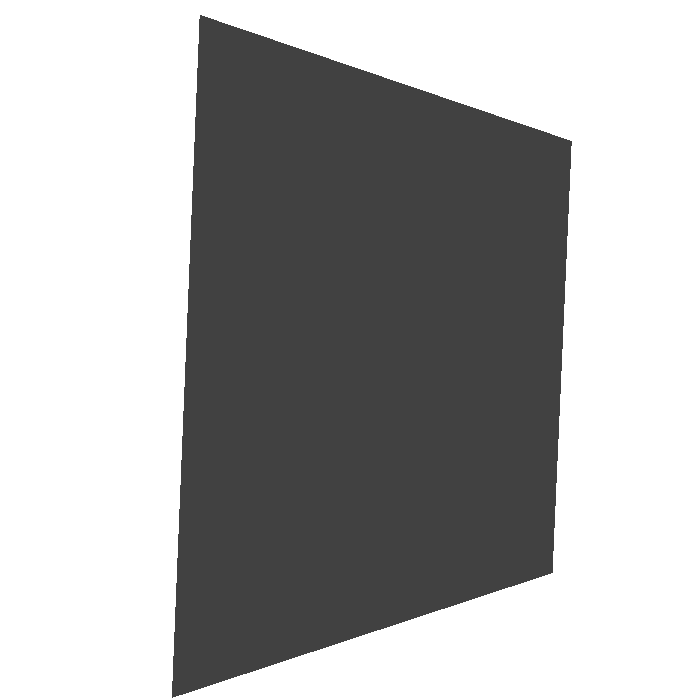
\includegraphics[height=0.18\textwidth]{./img/synthInit1}&
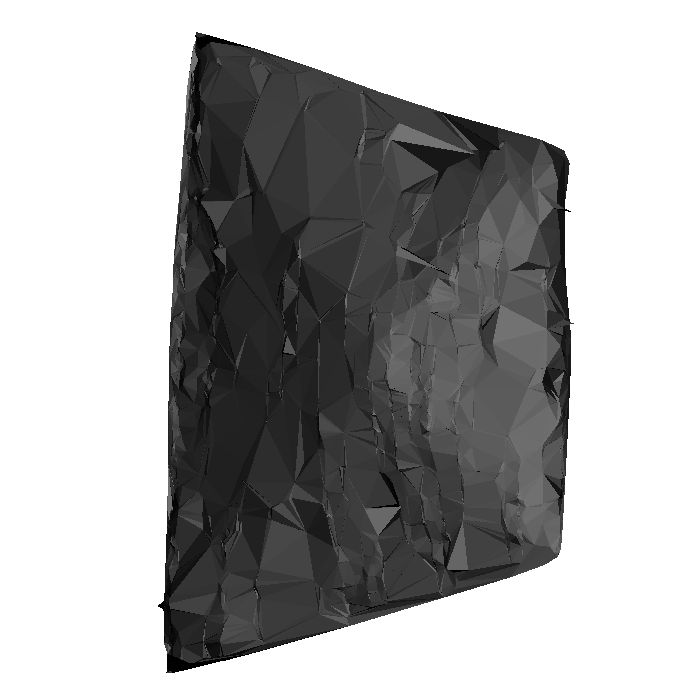
\includegraphics[height=0.18\textwidth]{./img/synthNOtRef1}&
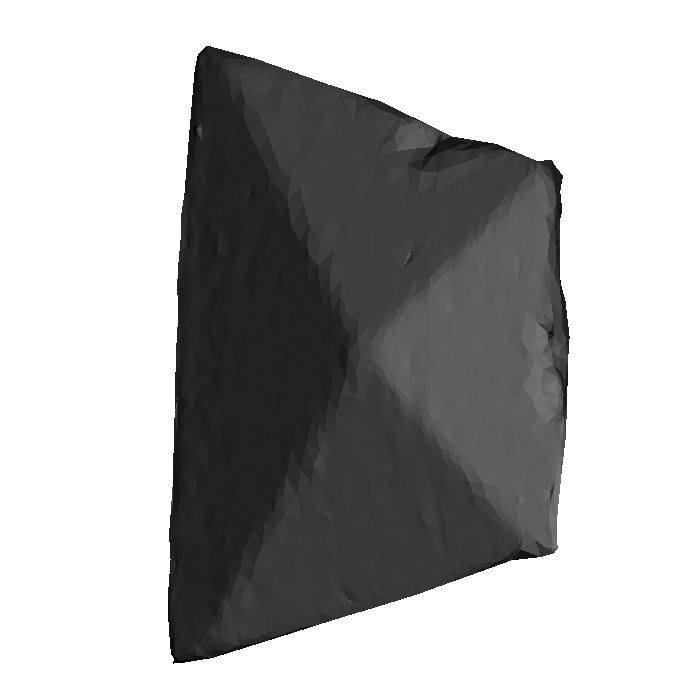
\includegraphics[height=0.18\textwidth]{./img/synthRef1}\\
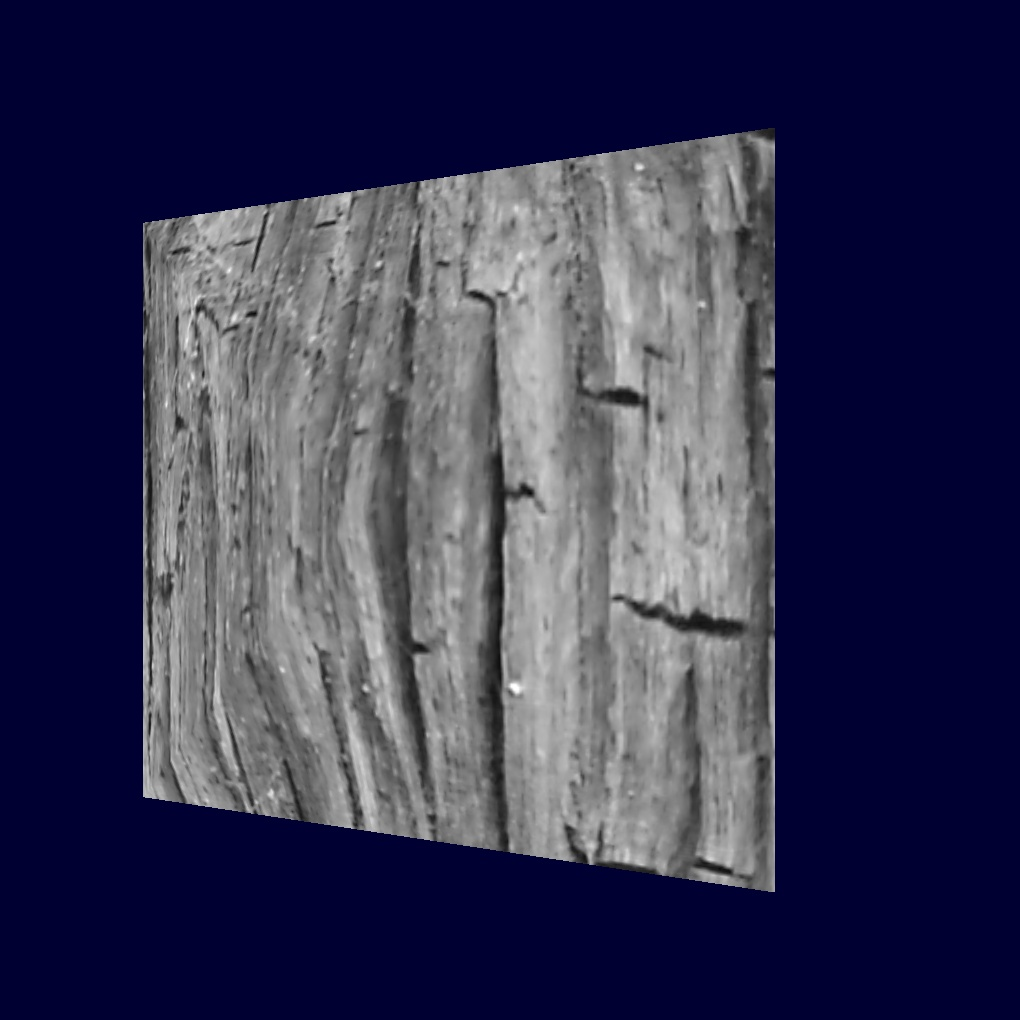
\includegraphics[height=0.18\textwidth]{./img/datasetSweepIMG1synth2}&
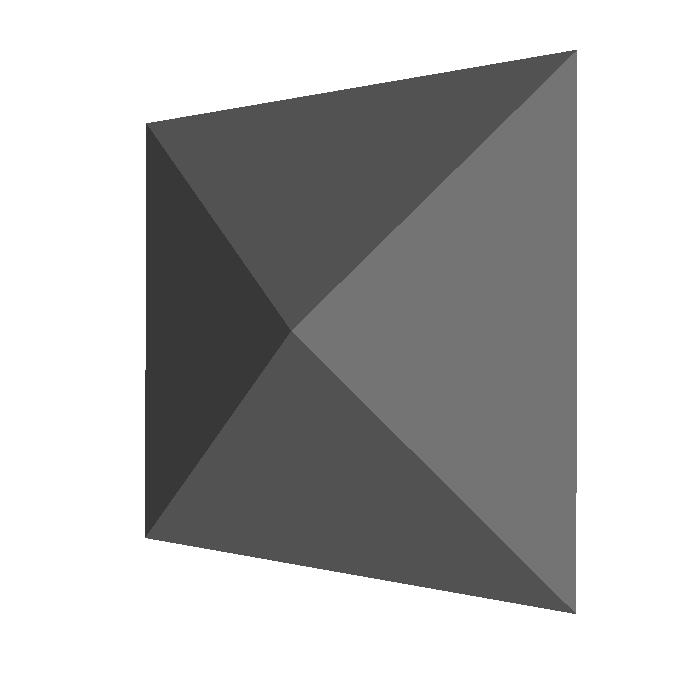
\includegraphics[height=0.18\textwidth]{./img/synth2_GT}&
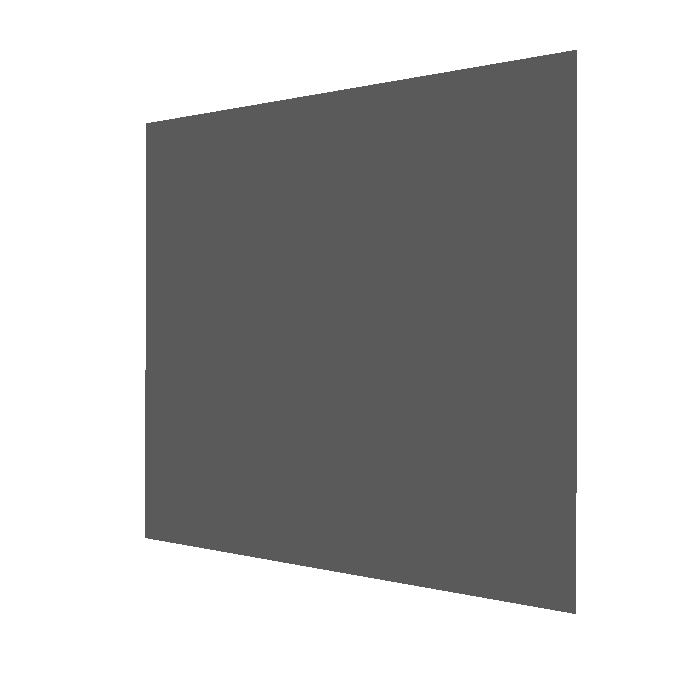
\includegraphics[height=0.18\textwidth]{./img/synth2_init}&
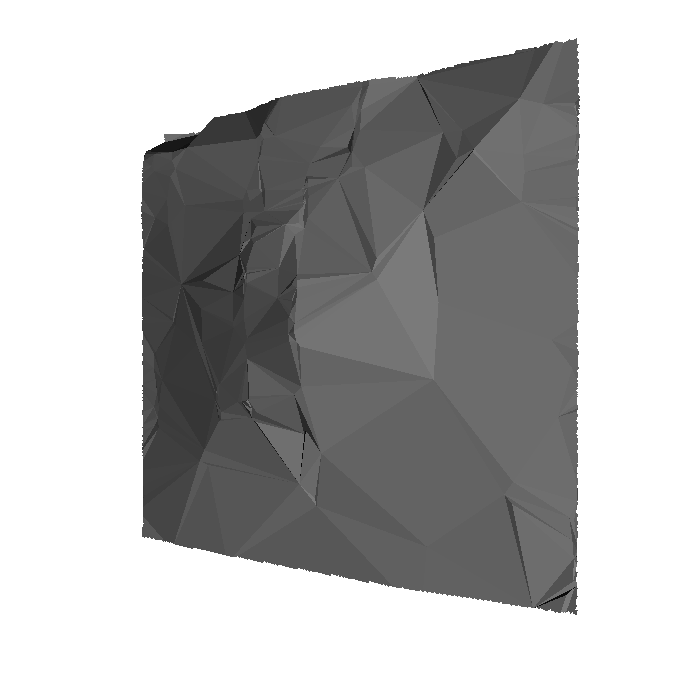
\includegraphics[height=0.18\textwidth]{./img/synth2_after_sweep}&
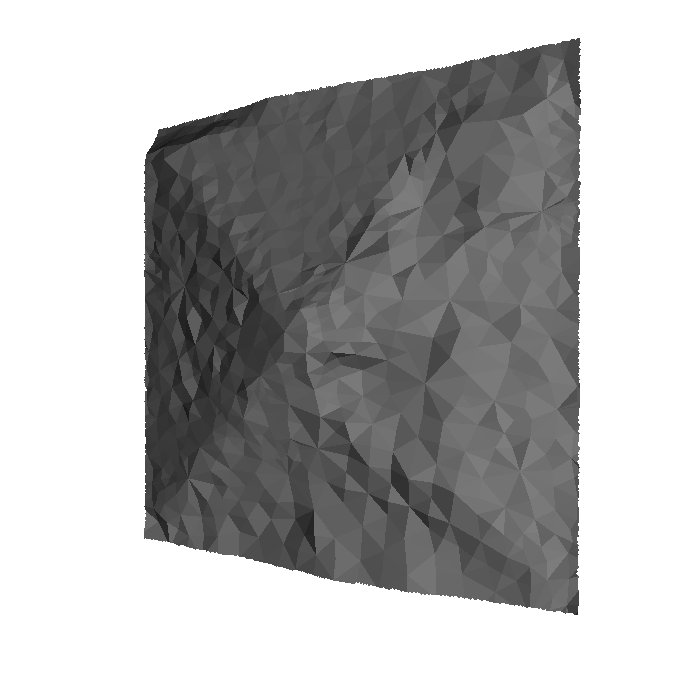
\includegraphics[height=0.18\textwidth]{./img/synth2_after_photo}\\
(a) &
(b)&
(c) &
(d) &
(e)\\
\end{tabular}
\caption{Simulated dataset results: (a) textured image, (b) ground-truth, (c) initial mesh, (d) after mesh sweeping, (e) after photometric refinement.}
\label{fig:simulated1}
\end{figure*}

The sweeping process produces a set of $N = 20$ meshes $\mathbb{M} = \{\mathcal{M}_1, \cdots, \mathcal{M}_j ,\cdots, \mathcal{M}_N\}$.
For each mesh $\mathcal{M}_j$ we perform pairwise stereo matching between each camera $C$ and the two nearest cameras.
Let $I_C$ be the image seen by $C$, and $I_k$ the image seen by the camera $C_k$, that is one of the two cameras nearest to $C$. 
We compute $I_k^j$ as the reprojection of image $I_k$ through the mesh $\mathcal{M}_j$ into camera $C$.

% We store in a second image $P_k^j$ the 3D position of the points that reproject for each pixels, such that $P_k^j(x,y)$ stores the 3D point nearest to camera $C$ that reprojects on pixel $(x,y)$.

Then, we compute  the Normalized Cross Correlation (NCC) image $I_C$ and the reprojection $I_k^j$. 
The NCC is computed pixel-by-pixel and is weighted by a Gaussian kernel as in \cite{pons2007multi}  (the $\sigma$ for the Gaussian kernel is $\sigma = 8 px$).

The last step aims at collecting the new 3D points. We create a $n_r$x$n_c$ grid over the $N$ images of pixel-by-pixel NCCs computed for each mesh $\mathcal{M}_j$. We collect in each tile the image point with the best NCC above a threshold $t_{\text{NCC}} = 0.98$ among all the $N$ images; therefore, we obtain at most $n_r$x$n_c$ points.
For each collected point, we retrieve its 3D position from the corresponding mesh that generated it.

We are able to perform the whole process image-based, i.e., we act on the image and not on the mesh, so that the most complex computations become independent from the size of the mesh, and they are self-adaptive with respect to the  image resolution. This also allows our approach to be adaptive in term of mesh resolution output.

% \subsection{Implementation details}
% We implemented our approach in C++ using the CGAL library \cite{cgal} for all the computations involving the Delaunay Triangulation and manifold extraction. This allows us to exploit efficiently data structures and algorithms for the initial manifold reconstruction tasks: thanks to the 3D triangulation module, we managed to encode all the visibility information inside each tetrahedron.
% 
% Conversely, the proposed mesh sweeping algorithms exploits the power of GPU computing. 
% We implemented the main steps with the GLSL shading language of OpenGL \cite{opengl}: a geometry shader computes the normal; the vertex shaders sweep the mesh along the camera viewing rays; the fragment shaders implement the reprojection from one image to an another through the mesh surface, the NCC computation and thresholding.
